\documentclass[a4paper,12pt]{thesis}

\usepackage[T1]{fontenc}
\usepackage{lipsum}
\usepackage{graphicx}

\usepackage{amsfonts}

\usepackage{xcolor}
\usepackage{hyperref}
\hypersetup{
    colorlinks=true,
    linkcolor=blue,
    citecolor=cyan,
    urlcolor=magenta,
}
\usepackage{url}
\usepackage[base]{babel}

\usepackage{cleveref}

\usepackage{algorithm}
\usepackage{algpseudocode}

\usepackage[natbib,style=ieee,refsection=chapter]{biblatex}

\addbibresource{01_indexing_intro.bib}
\addbibresource{02_fingerprint_indexing.bib}
% \addbibresource{03_vector_database.bib}
% \addbibresource{04_future_work.bib}


\title{Título do Documento}
\author{Seu Nome}
\date{\today}

\begin{document}

\maketitle

Teste

% \begin{abstract}
% Este é o resumo do documento.
% \end{abstract}

\chapter{Introdução à Indexação}

\section{O que é indexação?}

Um índice é uma estrutura de dados que melhora a velocidade das operações de query de dados em uma tabela, ao custo de escritas adicionais e espaço de armazenamento para manter a estrutura do índice. Índices permitem localizar dados rapidamente sem precisar buscar sequencialmente em cada linha de uma tabela.

A maioria dos softwares de banco de dados inclui tecnologia de indexação que permite buscas em tempo sub-linear para melhorar o desempenho, já que a busca linear é ineficiente para grandes bancos de dados.

\cite{databaseindex:wiki}

\section{Implementações de índices}

\subsection{B Tree}

Uma \textbf{B-tree} é uma estrutura de dados em árvore auto-balanceada que mantém dados ordenados e permite buscas, acessos sequenciais, inserções e deleções em tempo logarítmico. A B-tree generaliza a árvore binária de busca, permitindo nós com mais de dois filhos.

É amplamente utilizada em sistemas de arquivos e bancos de dados. É uma estrutura que se beneficia da leitura e escrita em bloco, levando vantagem em um aspecto historicamente relevante, uma vez que o número de operações de I/O (em discos magnéticos) era igualmente relevante para o desempenho quanto o número de operações de comparação.

Foi inventada por Rudolf Bayer e Edward M. McCreight em 1972 (o B não foi explicado por eles).

% Quote
\begin{quotation}
    \it What Rudy (Bayer) likes to say is, the more you think about what the B in B-Tree means, the better you understand B-Trees!
\end{quotation}

Os principais algoritmos associados a B-trees são: busca (\cref{alg:btree_search}) e inserção (\cref{alg:btree_insertion}) (existem variações para a operação de deleção).

São necessárias duas funções auxiliares para a inserção: \textsc{splitChild}, que divide um nó cheio em dois, e \textsc{insertNonFull}, que insere uma chave em um nó não cheio.

\begin{algorithm}
\caption{Algoritmo de busca na B Tree, assumindo que a chave $k$ é o valor a ser buscado e $x$ é o nó onde a busca começa.}
\label{alg:btree_search}
\begin{algorithmic}[1]
\Procedure{BtreeSearch}{$x, k$}
    \State $i \gets 0$
    \While{$i < x.n$ \textbf{and} $k > x.key[i]$}
        \State $i \gets i + 1$
    \EndWhile
    \If{$i < x.n$ \textbf{and} $k = x.key[i]$}
        \State \Return $x$
    \EndIf
    \If{$x.leaf$}
        \State \Return \textbf{None}
    \EndIf
    \State \Return \Call{BtreeSearch}{$x.child[i], k$}
\EndProcedure
\end{algorithmic}
\end{algorithm}

\begin{algorithm}
\caption{Algoritmo de inserção na B Tree, assumindo que a chave $k$ é o valor a ser inserido.}
\label{alg:btree_insertion}
\begin{algorithmic}[1]
\Procedure{BtreeInsert}{$T, k$}
    \State $r \gets T.root$
    \If{$r.n = 2(T.d) - 1$}
        \State $s \gets$ \textbf{new} Node
        \State $T.root \gets s$
        \State $s.child[1] \gets r$
        \State \Call{splitChild}{$s, 1$}
        \State \Call{insertNonFull}{$s, k$}
    \Else
        \State \Call{insertNonFull}{$r, k$}
    \EndIf
\EndProcedure
\end{algorithmic}
\end{algorithm}

\cite{btree:wiki}

\subsection{B+ Tree}

\cite{bptree:wiki}

\printbibliography

\chapter{Indexação para Fingerprints}

\section{Introdução}

\begin{itemize}
    \item Matching local baseado em minúcias
    \begin{itemize}
        \item Abordagens antigas \cite{automated:hrechak1990,finger:willis2001}
        \item Associa cada minúcia as suas vizinhas em estruturas invariantes a rotação e distâncias\cite{globallocal:jiang2000,robustlocal:ratha2000}
        \item Baseada em cilindros, veja \cref{sec:mcc}
        \item Outros métodos que incluem mais características: local orientation field, local frequency, ridge shapes
    \end{itemize}
\end{itemize}

Estruturas locais de uma minúcia central podem ser baseadas em:
\begin{itemize}
    \item \textit{Vizinhos mais próximos}, que consideram as $k$ minúcias mais próximas \cite{globallocal:jiang2000}.
    
    A vantagem dessa representação é com relação ao tamanho fixo, facilitando no procedimento de comparação.
    
    \item \textit{Raio fixo}, que considera todas as minúcias dentro de um raio fixo, usada em \cite{robustlocal:ratha2000}.
    
    A vantagem dessa representação é a tolerância com relação a ruído (minúcias extras ou faltantes).
\end{itemize}

\section{Minutia Cylinder-Code}
\label{sec:mcc}

Baseada em \cite{mccmatching:cappelli2010,mccindexing:cappelli2010}

\subsection{Representação}

Uma representação tridimensional de minúcias baseada em distâncias entre minúcias e ângulos relativos. A representação recebe o nome de Minutia Cylinder-Code (MCC) e tem como características principais: invariância de rotação, tamanho fixo e orientada a codificação binária.

O esquema de representação é um cilindro segmentado, como na \cref{fig:mcc}. O cilindro é um recorte de um cubo dividido em células, onde cada uma possui um valor indexado por $C_m[i, j, k]$.

\begin{figure}
    \centering
    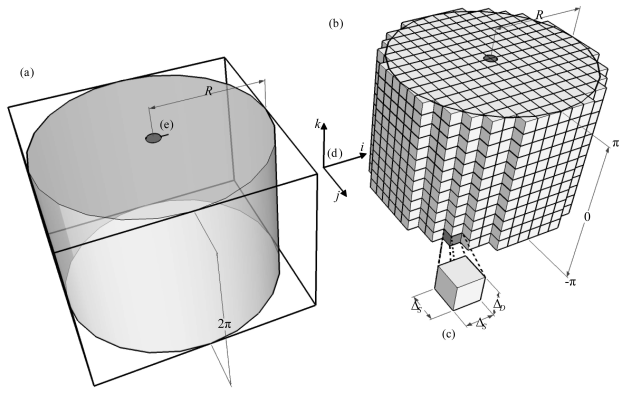
\includegraphics[width=0.6\textwidth]{imgs/fingerprint_cylinder_code.png}
    \caption{Representação de um MCC.}
    \label{fig:mcc}
\end{figure}

O cálculo dos valores de $C_m[i, j, k]$ é complicado, mas essencialmente envolve as seguintes ideias:
\begin{itemize}
\item Verifica se está em uma região válida: dentro do cilindro e dentro do \textit{convex hull} da fingerprint.
\item Calcula a contribuição de cada minúcia vizinha usando uma Gaussiana, \cref{fig:mccdist}.
\item Calcula a contribuição de cada minúcia usando a diferença entre a orientação.
\end{itemize}

\begin{figure}
    \centering
    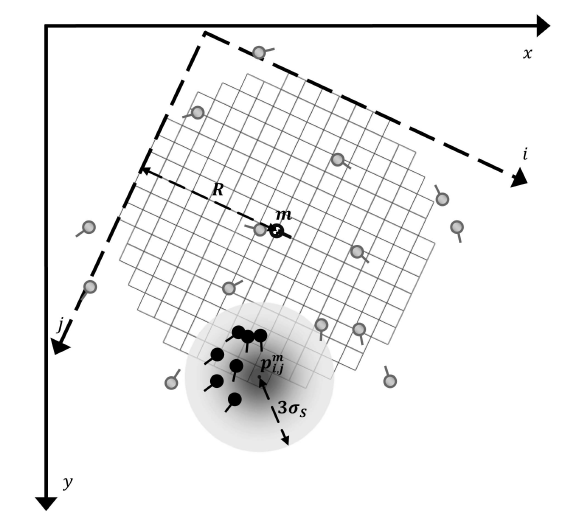
\includegraphics[width=0.6\textwidth]{imgs/eval_cylinder.png}
    \caption{Contribuição da distância de uma minúcia vizinha. Cores mais escuras refletem uma maior contribuição.}
    \label{fig:mccdist}
\end{figure}

\subsection{Similaridade}

A similaridade entre dois cilindros é obtida a partir do seguinte procedimento:
\begin{enumerate}
    \item Lineariza o cilindro em um vetor, similar a operação de \texttt{reshape}. Por exemplo, o cilindro de uma minúcia $a$, $C_a[i, j, k]$, é linearizado em $\mathbf{c}_a$.
    \item Seleciona todas as entradas comparáveis desses vetores (células que são \textit{válidas} em ambos) que dão origem aos vetores $\tilde{\mathbf{v}}_a$ e $\tilde{\mathbf{v}}_b$.
    \item Na implementação binária, é realizado um XOR bit a bit entre os vetores.
    \begin{equation}
        \gamma(\tilde{\mathbf{v}}_a, \tilde{\mathbf{v}}_b) =
            1 - \frac{\|\tilde{\mathbf{v}}_a \oplus \tilde{\mathbf{v}}_b\|}{\|\tilde{\mathbf{v}}_a\| + \|\tilde{\mathbf{v}}_b\|}
    \end{equation}
\end{enumerate}

\subsection{Indexação}

Para a indexação de um MCC é empregado um esquema de \textit{locality-sensitive hashing} (LSH).

O procedimento consiste em:
\begin{enumerate}
    \item Seja $\mathbf{v}_m$ o vetor obtido da linearização de um cilindro.
    \item É feita a projeção de $\mathbf{v}_m$ em um subespaço $\mathbf{h}_m$. A projeção é obtida simplesmente ao escolher um subconjunto dos índices $H$ do vetor original.
    \begin{equation}
        \mathbf{h}_m = \mathbf{v}_m[H]
    \end{equation}
    \item O conjunto $H$ define uma função que mapeia um vetor binário $\mathbf{v}_m$ em um número natural obtido ao interpretar o vetor binário $\mathbf{h}_m$ como um número natural.
    \begin{equation}
        h_H: \{0, 1\}^n \rightarrow \mathbb{N}
    \end{equation}
    \item São definidos $\ell$ conjuntos $H_1, H_2, \ldots, H_\ell$, cada um com uma função $h_{H_i}$.
    \item O índice por sua vez é um conjunto de \textit{hash tables}, $\mathbb{H}_1, \mathbb{H}_2, \ldots, \mathbb{H}_\ell$, onde cada hash table tem os seus buckets definidos pela função $h_{H_i}$.
    \item A indexação segue fazendo a consulta do vetor desejado em cada hash table, retornando os candidatos.
    \item Por fim, os candidatos são ranqueados usando a \textit{distância de Hamming} entre os vetores.
\end{enumerate}

O procedimento enumerado acima é ilustrado na \cref{fig:lshmcc}.

\begin{figure}
    \centering
    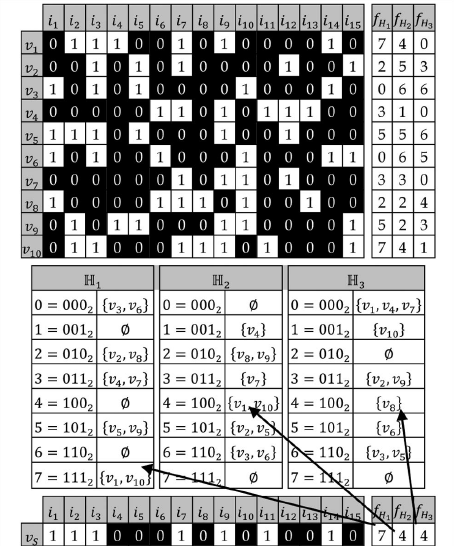
\includegraphics[width=0.8\textwidth]{imgs/cylinder_lsh.png}
    \caption{Ilustração do procedimento de indexação usando LSH de um MCC.}
    \label{fig:lshmcc}
\end{figure}

\printbibliography

% \chapter{Vector Databases}

\section{Introdução}

Os chamados \textit{Vector Databases} (VDB) surgem em um cenário no qual \textit{dados não estruturados} são dominantes em praticamente todas as esferas e as previsões apontam para um crescimento contínuo e acelerado. Exemplos de dados dessa forma são aqueles que não podem ser armazenados de forma padronizada em tabelas, como imagens, vídeos, áudios e textos.

Para contrapor a definição de dados não estruturados, entende-se por \textit{dados estruturados} aqueles que podem ser colocados em forma de tabelas, como aqueles armazenados em bancos de dados relacionais. Define-se também os \textit{dados semi-estruturados}, que são aqueles que possuem uma estrutura menos rígida, como arquivos XML e JSON.

A mudança de paradigmas apresentadas pelos dados não estruturados diz respeito a como deve ser feita a interpretação desses dados. Diferentes imagens de cachorros são objetivamente diferentes analisando o seu conteúdo bruto (valor dos pixels), mas todas as imagens apresentam uma \textit{similaridade semântica}. O desafio passa a ser então como representar, armazenar e realizar busca nesses dados, de forma que eles reflitam esse aspecto.

A abordagem que segue é a de representar os dados por meio de métodos de \textit{aprendizado profundo}, gerando a partir de um pedaço de dado não estruturado um vetor multidimensional, chamado de \textit{embedding}. Observa-se na literatura que uma rede neural bem treinada é capaz de capturar a semântica desses dados e, portanto, a similaridade entre eles é refletida por uma medida de distância entre os vetores.

\subsection{Aplicações}

...

\section{Divisão dos métodos}

\begin{itemize}
    \item Busca exata
    \begin{itemize}
        \item Linear Scan
        \item Space Partitioning (KD-Tree, Ball-Tree, Inverted File Index)
    \end{itemize}
    \item Busca aproximada
    \begin{itemize}
        \item Cluster-based
        \item Graph-based
        \item Tree-based
        \item Hash-based 
    \end{itemize}
    \item Quantização
    \begin{itemize}
        \item Scalar Quantization
        \item Product Quantization
    \end{itemize}
\end{itemize}

\section{Métodos exatos}

\subsection{Linear Scan}

O algoritmo de busca linear, \textit{flat indexing}, calcula a distância entre a query $Q$ e todos os elementos do conjunto de dados $\mathcal{D}$, retornando o elemento mais próximo. A complexidade desse algoritmo é $O(n)$, onde $n$ é o número de elementos em $\mathcal{D}$, tornando-o muitas vezes impraticável em cenários reais. O algoritmo é apresentado no \cref{alg:linear_scan}.

\begin{algorithm}
\caption{Algoritmo de busca linear de uma query $Q$ em um conjunto de dados $\mathcal{D}$.}
\label{alg:linear_scan}
\begin{algorithmic}[1]
\Procedure{LinearScan}{$Q$, $\mathcal{D}$}
    \State $best\_dist \gets \infty$
    \State $best\_match \gets \text{None}$
    \For{$d \in \mathcal{D}$}
        \State $dist \gets \text{dist}(Q, d)$
        \If{$dist < best\_dist$}
            \State $best\_dist \gets dist$
            \State $best\_match \gets d$
        \EndIf
    \EndFor
    \State \Return $best\_match$
\EndProcedure
\end{algorithmic}
\end{algorithm}

\subsection{Particionamento de Espaço}

Métodos exatos de busca podem ser vistos em \cref{sec:multidimsearch}.

O que acontece nesses caso é a maldição da dimensionalidade. Sendo assim, métodos de busca aproximados devem ser utilizados, trocando um pouco de precisão por eficiência.

\section{Métodos baseados em clusterização}

\subsection{Inverted File Index (IVF)}

A estratégia de IVF é baseada em dividir o espaço em partições, representadas a partir do centroide de todos os vetores que pertencem a essa partição.

Os centroides de cada partição, ou \textit{clusters}, são determinados pelo algoritmo de clusterização \textit{$k$-means}. O funcionamento desse algoritmo consiste em: inicialmente selecionar aleatoriamente $k$ vetores do conjunto de dados e atribuir a cada um deles um cluster; em seguida adicionar a cada cluster os vetores mais próximos a ele; atualizar o novo centroide de cada cluster; repetir o processo até a convergência \cite{kmeans:wiki, lloydsalg:wiki}.

A busca, dessa forma, pode ser limitada somente aos vetores que pertencem a uma partição ou conjunto de partições, reduzindo o espaço de busca, como ilustra \cref{alg:ivf}.

\begin{algorithm}
\caption{Algoritmo de busca usando o IVF de uma query $Q$ em um índice $\mathcal{I}$.}
\label{alg:ivf}
\begin{algorithmic}[1]
\Procedure{IVFSearch}{$\mathcal{I}, query, top\_k, nprobe$}
    \State $distances \gets []$
    \ForAll{$c \in \mathcal{I}.centroids$}
        \State $d \gets \|query - c\|$
        \State $distances \gets distances \cup \{(c, d)\}$
    \EndFor
    \State $candidateCentroids \gets$ \textbf{selecionar os $nprobe$ menores} $d$
    \State $candidateVectors \gets \{\}$
    \ForAll{$ctr \in candidateCentroids$}
        \State $candidateVectors \gets candidateVectors \cup \mathcal{I}[ctr]$
    \EndFor
    \State $scored \gets []$
    \ForAll{$v \in candidateVectors$}
        \State $dist \gets \|query - v\|$
        \State $scored \gets scored \cup \{(v, dist)\}$
    \EndFor
    \State ordenar $scored$ \textbf{por} $dist$ \textbf{ascendente}
    \State \textbf{return} \textbf{primeiros} $top\_k$ \textbf{de} $scored$
\EndProcedure
\end{algorithmic}
\end{algorithm}

\section{Métodos baseados em grafos}

\subsection{Navigable Small World}

A princípio\cite{scalable:malkov2012,smallworldgraphs:malkov2014} o autor, Yury Malkov, estava interessado no problema de vizinhos mais próximos em uma configuração distribuída.

Quais as vantagens apontadas para essa escolha?
\begin{itemize}
    \item Existem algoritmos para construir essas redes,
    \item Não tem elementos raízes,
    \item Operações de adição e busca usam somente informações locais e podem ser iniciadas de qualquer elemento.
\end{itemize}

\begin{quotation}
    \it This gives an opportunity for building decentralized similarity search oriented storage
    systems where physical data location doesn't depend on the content because every
    data object can be placed on an arbitrary physical machine and can be connected with
    others by links like in p2p systems.
\end{quotation}

Uma das técnicas de busca em grafos com vértices contendo elementos de um espaço métrico é a busca gulosa. Nesse caso, para que a busca seja exata, i.e., encontra sempre os verdadeiros vizinhos mais próximos, é necessário que o grafo contenha o grafo de Delaunay como subgrafo ({\color{purple}dual a tesselação de Voronoi}). As limitações da busca exata estão associadas a necessidade de conhecimento prévio da estrutura interna do espaço\cite{searching:navarro2002} e a maldição da dimensionalidade \cite{voronoi:aurenhammer1991}. Caso a condição de busca exata seja relaxa, é necessário conter somente uma aproximação do grado de Delaunay.

Para que a busca gulosa tenha escalabilidade logarítmica, a rede small world deve ter a propriedade de ser \textit{navegável}.\cite{smallworld:kleinberg2000}

As arestas $E$ da rede são divididas em dois grupos: arestas de baixo alcance, que aproximam o grafo de Delaunay e responsáveis pelo resultado do roteamento guloso, e as arestas de longo alcance, que servem para fornecer a escalabilidade logarítmica da busca gulosa devido a propriedade de navigabilidade.

% Figure
\begin{figure}
    \centering
    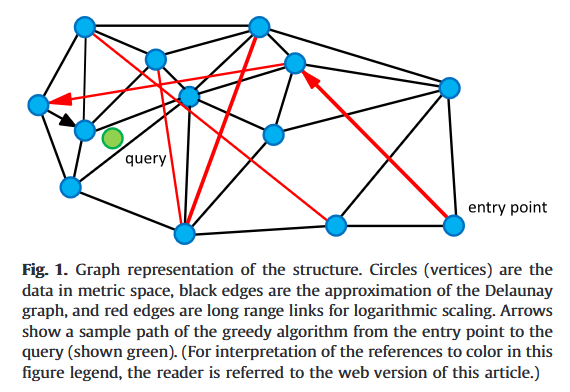
\includegraphics[width=0.7\textwidth]{imgs/navigablesmallworld_graph.png}
    \label{fig:navsmallworld}
\end{figure}

\subsubsection{Busca}

O algoritmo \cref{alg:buscagulosa} encontra o objeto no conjunto de dados mais próximo ou um falso mais próximo. Caso todo o elemento na estrutura tivesse em sua lista de vizinhos todos os vizinhos no sentido de Voronoi, isso seria a condição para o grafo de Delaunay e da busca exata.

\begin{algorithm}
\caption{Busca gulosa em busca de um mínimo local em um grafo Small World.}
\label{alg:buscagulosa}
\begin{algorithmic}[1]
\Procedure{GreedySearch}{$q, ep$}
    \State $curr \gets ep$
    \State $dmin \gets d(q, curr)$
    \State $next \gets \text{Null}$
    \ForAll{$n \in curr.neighbors$}
        \If{$d(q, n) < dmin$}
            \State $dmin \gets d(q, n)$
            \State $next \gets n$
        \EndIf
    \EndFor
    \If{$next = \text{Null}$}
        \State \Return $curr$ \Comment{Reached local minima}
    \Else
        \State \Return \Call{GreedySearch}{$q, next$}
    \EndIf
\EndProcedure
\end{algorithmic}
\end{algorithm}

Uma estratégia para diminuir o erro, \cref{fig:nsw_falsepositive} é realizar um conjunto de $m$ buscas independentes, começando de pontos distintos, e retornar o melhor resultado. Caso a probabilidade de encontrar o mínimo global seja $p$, então a probabilidade de encontrar o mínimo global em pelo menos uma das buscas é $1 - (1 - p)^m$, indicando que a probabilidade de falha decai exponencialmente com o número de buscas.

\begin{figure}
    \centering
    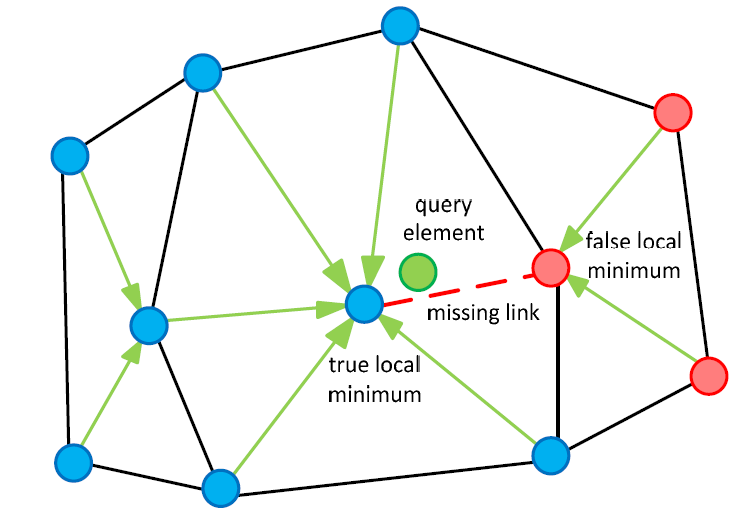
\includegraphics[width=0.7\textwidth]{imgs/nsw_falsepositive.png}
    \caption{Caso ilustrativo de um falso positivo na busca gulosa.}
    \label{fig:nsw_falsepositive}
\end{figure}

\begin{algorithm}
\caption{MultiSearch}
\begin{algorithmic}[1]
\Procedure{MultiSearch}{$q, m$}
    \State $candidatos \gets []$
    \For{$i \gets 1$ \textbf{to} $m$}
        \State $ep \gets$ \Call{getRandomEntryPoint}{}
        \State $result \gets$ \Call{GreedySearch}{$q, ep$}
        \State $candidatos \gets candidatos \cup \{result\}$
    \EndFor
    \State ordenar $candidatos$ \textbf{por} $d(q, \cdot)$ \textbf{ascendente}
    \State \Return $candidatos$
\EndProcedure
\end{algorithmic}
\end{algorithm}

Em \cite{smallworldgraphs:malkov2014}, o algoritmo é refinado. Nova condição de parada: as iterações ocorrem somente em não visitados, para quando o próximo elemento não altera os $k$ mais próximos.

\subsubsection{Construção}

Sabendo que o objetivo é construir somente uma aproximação do grafo de Delaunay, existe grande liberdade na etapa de construção. Existe um método que busca minimizar o volume das células de Voronoi por Monte Carlo. O método proposto é construir o grafo de forma iterativa, uma adição por vez.

Usando a ideia de 
\textsc{MultiSearch}, podemos fazer o seguinte procedimento, ilustrado em \cref{alg:nsw_add}, obter um conjunto de mínimos locais a partir de $m$ buscas, ordenar os resultados pela distância com o objeto inserido e conectar os $k$ mais próximos.

\begin{algorithm}
\caption{Adição de um novo objeto ao grafo Small World.}
\label{alg:nsw_add}
\begin{algorithmic}[1]
\Procedure{kNN-Add}{$q, m, k$}
\State $localMins \gets$ \Call{MultiSearch}{$q, m$}
\State $vizinhos \gets []$
\ForAll {$lm \in localMins$}
    \State $vizinhos \gets vizinhos \cup \{lm\}$
\EndFor
\State ordenar $vizinhos$ \textbf{por} $d(q, \cdot)$ \textbf{ascendente}
\For{$i \gets 1$ \textbf{to} $k$}
    \State \Call{Connect}{$q, vizinhos[i]$}
\EndFor
\EndProcedure
\end{algorithmic}
\end{algorithm}

A ideia por trás disso é que a intersecção entre os vizinhos de Voronoi e os k vizinhos mais próximos deve ser grande. Além disso, com dados chegando de forma aleatória, a característica de navigabilidade é obtida sem passos adicionais (os primeiros elementos tendem a gerar os links de longo alcance).

\subsubsection{Resultados}

\begin{itemize}
    \item Verifica propriedade de navigabilidade do Small World: medir o tamanho médio do caminho percorrido durante a busca. De fato, é logaritmico com relação ao tamanho do dataset.
    \item Número de buscas do \textsc{MultiSearch}: Para manter uma taxa de acerto de $p=.95$, mostrou-se que $m>A\log n$. Isso mostra que o número de buscas, durante a fase de construção, para obter um valor alto de $p$ cresce de forma logarítmica.
    \item Número de conexões ($k$): Aproximadamente $3d$, que mantém baixa taxa de erro para uma baixa taxa de elementos visitados durante a busca.
    \item Fração de elementos visitados: Diminui com aumento do dataset. A relação entre número de elementos e porcentagem de visitados é, em escala log-log, uma reta com inclinação de -45 graus, $\text{porcentagem} = -kn^{-1}$.
    \item Complexidade da busca (tamanho dataset): É $\log^2 n$, sendo um ``log'' do tamanho do caminho e outro do número de ``buscas''.
    \item Complexidade da busca (dimensão): É $d^{1.7}$.
\end{itemize}

No geral, complexidade de busca
$$O(d^{1.7}\log^2n \log(1/p_\text{fail}))$$
de construção é
$$O(d^{1.7}n\log^2n)$$

\subsection{Hierarchical Navigable Small World (HNSW)}

Em grafos de proximidade, sofrem de problemas de escalabilidade por lei de potência e possível desconexão global em dados clusterizados. Soluções envolvendo uma etapa de busca grosseira (coarse search) usando outras estruturas para definir o ponto de entrada foram sugeridas.

Nos trabalhos anteriores, um grafo de proximidade com a característica de navegabilidade (grafo NSW) foi proposto. Essas estruturas apresentam escalabilidade logarítmica ou polilogarítmica no número de saltos durante a busca com relação ao tamanho do grafo. O método é baseado na construção incremental da estrutura, sempre ligando um novo elemento ao conjunto de $k$ elementos mais próximos. Para encontrar os $k$ mais próximos, são feitas múltiplas buscas a partir de pontos de entrada diferentes. Conexões antigas, servem como conexões de longo alcance que permite a escalabilidade logarítmica.

No entanto, a escalabilidade polilogarítmica do número de cálculos de distância na busca era uma limitação. Essa escalabilidade é devido a: $\langle\text{\# hops}\rangle\times \langle\text{node degree}\rangle$. O primeiro termo é logaritmico como discutido e o segundo também, devido ao fato do número de hubs crescer logaritmicamente com o tamanho do grafo.

Para melhorar o método, 
\begin{itemize}
    \item começar em um nó com alto grau, para evitar ficar preso em um mínimo local. Os nós iniciais são ideais para isso e aumentam a chance de um roteamento bem sucedido. 
    \item dividir o grafo segundo a distância das conexões. Dessa maneira, fixando o número de conexões avaliadas para um número constante, permitindo o tempo geral logaritmico.
\end{itemize}

A essência desse novo método\cite{hnsw:malkov2018} é começar na camada mais superior, que apresentam os maiores links, realizar uma busca gulosa até um mínimo local e continuar a busca a partir desse mesmo elemento na camada inferior, repetindo o processo, \cref{fig:hnsw}.

\begin{figure}
    \centering
    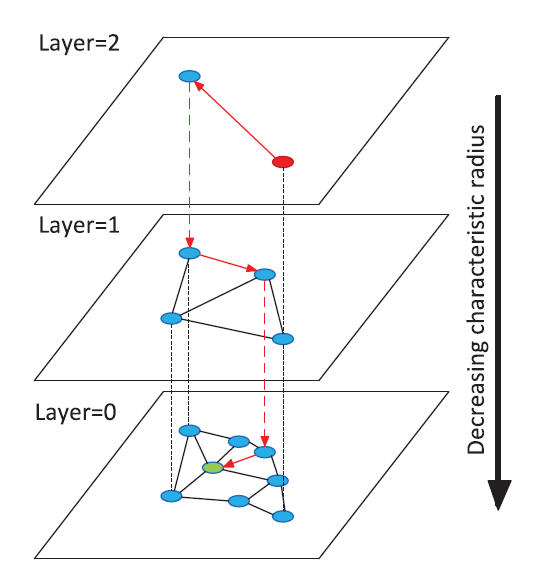
\includegraphics[width=0.6\textwidth]{imgs/hnsw.png}
    \caption{Hierarchical Navigable Small World.}
    \label{fig:hnsw}
\end{figure}

Para construir essa estrutura por camadas é sortear o nível máximo que um elemento vai ocupar usando uma distribuição exponencial. A criação de links também usa uma heurística para diversificar as conexões.

\subsubsection{Construção}

\cref{alg:hnsw_insert}.

$O(n \log n)$

\begin{algorithm}
\caption{Inserção de um elemento.}
\label{alg:hnsw_insert}
\begin{algorithmic}[1]
\Procedure{Insert}{$q, M, M_\text{max}, efConstruction, m_L$}
\State $\text{NN} \gets []$
\State $ep \gets hsnw.ep$
\State $L \gets ep.level$
\State $l \gets \lfloor-m_L\ln\mathcal{U}(0, 1)\rfloor$
\For{$l_c \gets L$ \textbf{to} $l + 1$}
\Comment{Camadas nas quais não está presente...}
\State $\text{NN} \gets$ \Call{SearchLayer}{$q, ep, ef=1, l_c$}
\State $ep \gets$ nearest element in $\text{NN}$ to $q$
\EndFor
\For{$l_c \gets \min(l, L)$ \textbf{to} $0$}
\State $\text{NN} \gets$ \Call{SearchLayer}{$q, ep, efConstruction, l_c$}
\State $vizinhos \gets $\Call{SelectNeighbors}{$q, \text{NN}, M, l_c$}
\State \Call{Connect}{$q, vizinhos$} no nível $l_c$
\ForAll{$v \in vizinhos$}
\If{$v.neighbors(l_c) > M_\text{max}$}
\State $novos \gets$ \Call{SelectNeighbors}{$v, v.neighbors(l_c), M_\text{max}, l_c$}
\State $v.neighbors(l_c) \gets novos$
\EndIf
\EndFor
\State $ep \gets \text{NN}$
\Comment{$ep$ pode ser uma lista de elementos}
\EndFor
\If{$L < l$}
\State $hsnw.ep \gets q$
\EndIf
\EndProcedure
\end{algorithmic}
\end{algorithm}

\subsubsection{Busca}

\cref{alg:hnsw_searchlayer}.

A complexidade de uma única busca pode ser obtida considerando que construímos um grafo de Delaunay exato e, então, o elemento selecionado em um dado nível é o mais próximo. Ao selecionar um elemento, a probabilidade dele estar no próximo nível é $p = \exp(-m_L)$. No entanto, durante a busca nesse nível, se são realizados $s$ passos, então esses $s$ elementos não podem estar no nível acima, pois caso contrário eles seriam retornados.

Agora considerando que para alcançar o melhor elemento são necessários $s$ passos, então a probabilidade de não alcançar o elemento é limitada por $p^s = \exp(-m_Ls)$. O número esperado ???

$O(\log n)$

\begin{algorithm}
\caption{Busca dos $ef$ elementos mais próximos de uma query $q$ em uma camada.}
\label{alg:hnsw_searchlayer}
\begin{algorithmic}[1]
\Procedure{SearchLayer}{$q, ep, ef, l_c$}
\State $visitados \gets \{ep\}$
\State $candidatos \gets \{ep\}$
\State $\text{NN} \gets []$
\While{$candidatos \neq \emptyset$}
\State $proximo \gets$ \textbf{pop} $candidatos$
\State $distante \gets \text{NN}.last$
\If{$\|q - proximo\| > \|q - distante\|$}
\State \textbf{break}
\EndIf
\For{$v \in proximo.neighbors(l_c)$}
\If{$v \notin visitados$}
\State $visitados \gets visitados \cup \{v\}$
\State $distante \gets \text{NN}.last$
\Comment{Atualiza o mais distante}
\If{$\|q - v\| < \|q - distante\|$ \textbf{or} $\text{NN}.\text{size} < ef$}
\State $candidatos \gets candidatos \cup \{v\}$
\State $\text{NN} \gets \text{NN} \cup \{v\}$
\If{$\text{NN}.\text{size} > ef$}
\State remove o mais distante de $\text{NN}$
\EndIf
\EndIf
\EndIf
\EndFor
\EndWhile
\State \Return $\text{NN}$
\EndProcedure
\end{algorithmic}
\end{algorithm}

\subsubsection{Escolhendo os vizinhos}

A maneira mais simples é escolher os vizinhos mais próximos. A outra é adotando uma heurística \cref{fig:hnsw_heuristic} que cria conexões em direções diversas, levando em conta a distância entre candidatos.
A heurística analisa os candidatos, começando do mais próximo, e escolhe para fazer a conexão somente aqueles que são mais próximos do objeto inserido $q$ do que dos outros candidatos inseridos.

\begin{algorithm}
\caption{Seleção de vizinhos via heurística.}
\begin{algorithmic}[1]
\Procedure{SelectNeighbors}{$q, candidatos, M, l_c$}
\State todo...
\EndProcedure
\end{algorithmic}
\end{algorithm}

\begin{figure}
    \centering
    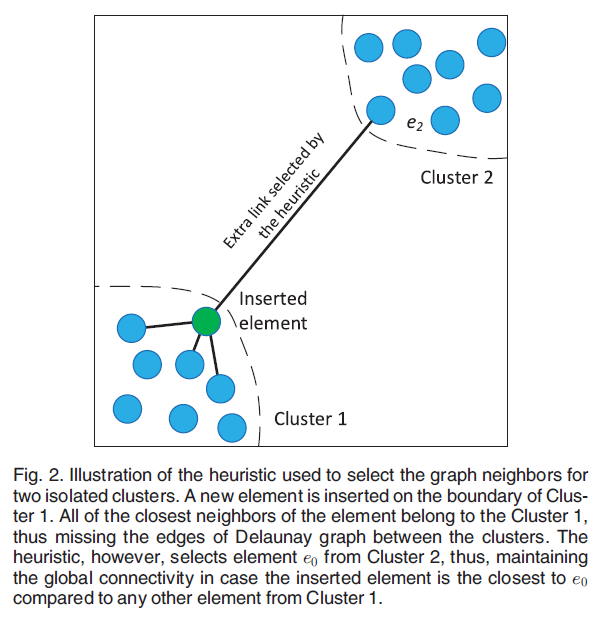
\includegraphics[width=0.7\textwidth]{imgs/hnsw_heuristic.png}
    \caption{Heurística de seleção de vizinhos.}
    \label{fig:hnsw_heuristic}
\end{figure}

\subsubsection{Parâmetros}

Os parâmetros que dão as características principais dos métodos quando comparados aos anteriores são $m_L$ e $M_\text{max}$. Se $m_L=0$ e $M_\text{max}=M$, é um grafo kNN com escalabilidade dada por lei de potência. Se $m_L=0$ e $M_\text{max}=\infty$ é um grafo NSW com escalabilidade polilogarítmica. Ao escolher $m_L>0$, passa a ser possível controlar a hierarquia do grafo, com a escalabilidade logarítmica.



\section{Métodos baseados em árvores}

\subsection{Approximate Nearest Neighbors Oh Yeah (ANNOY)}

\section{Métodos baseados em hashing}

\subsection{LSH}

\section{Quantização}

A quantização busca diminuir o tamanho do banco de dados, representando os vetores por suas representações quantizadas. Note que isso é diferente do método de redução de dimensionalidade, como (PCA, t-SNE, UMAP).

\subsection{Scalar Quantization}

Transforma vetores de floats em vetores de inteiros. Para cada dimensão, o método busca todo o alcance e divide essa faixa uniformemente em bins. Se queremos armazenar o inteiro em um \texttt{uint8}, então temos $2^8 = 256$ bins.

\subsection{Product Quantization}

Dado um vetor que possui $d$ bits. Cada vetor é dividido em $m$ subvetores, cada um com $d/m$ bits. Em seguida, para todos os subvetores, é feita uma clusterização por $k$-means. Substituímos todos os subvetores por seus respectivos centroides.


\section{Opções comerciais}





\printbibliography

% \chapter{Trabalhos Futuros}

% Use lipsum for dummy text
\lipsum[1-2]

\cite{dirac}

\printbibliography

\end{document}